\subsection{Architecture}
\begin{figure}[H]
    \centering
    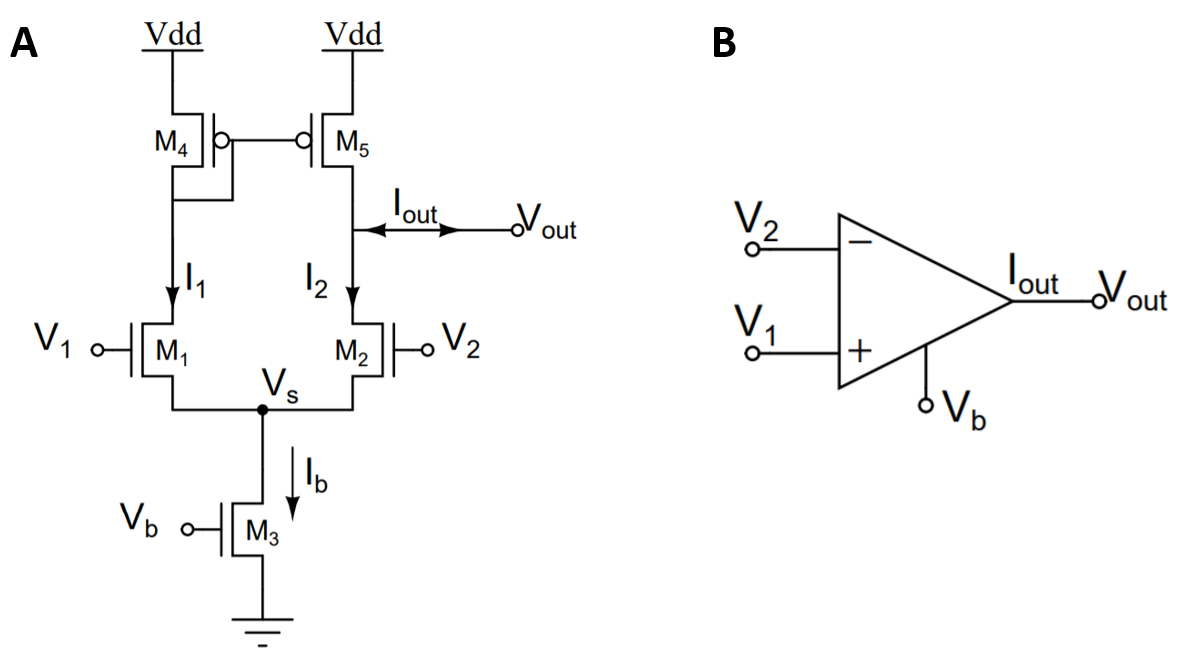
\includegraphics[width=0.8\linewidth]{../../Figures/Transconductance_Amplifier.PNG}
    \caption{The Transconductance Amplifier. A) Transconductance Amplifier Circuit. B) Electrical symbol of the Transconductance Amplifier. Adapted from Lecture Notes.}
    \label{fig:transconductance_amplifier}
\end{figure}

In the Transconductance Amplifier circuit, shown in Figure \ref{fig:transconductance_amplifier}.A, the first thing to pay attention to is that it is a combination to two circuits we have studied before: the differential pair (on the lower end) and a P-Type current mirror (on the higher end). Let's remind ourselves of the important equations and assumptions of the diff pair and the P-type current mirror. 
\newline
\paragraph{The differential pair} Remember that the differential pair implements a difference between the two input voltages $V_1$ and $V_2$ which translates to the two output currents $I_1$ and $I_2$. Here are the equations:

\begin{equation}
    I_1 = I_b\frac{e^{\kappa_n V_1/U_T}}{e^{\kappa_n V_1/U_T + e^{\kappa_n V_2/U_T}}}
\end{equation}
\begin{equation}
    I_2 = I_b\frac{e^{\kappa_n V_2/U_T}}{e^{\kappa_n V_1/U_T + e^{\kappa_n V_2/U_T}}}
\end{equation}

We previously assumed that all transistors work in subtreshold and saturation Remember also the sigmoid behaviour of the two output currents, as well as the hyperbolic tangent (tanh) behaviour of the difference between the two currents. 

\paragraph{The P-type current mirror}

We have shown in the previous chapter that the P-Type current mirror behaves as follows: 

\begin{equation}
I_{out} = I_{in} e^{\frac{V_{s_1} - V_{s_2}}{U_T}}
\end{equation}

In our case, both $V_{S_1}$ and $V_{S_2}$ are $V_{dd}$. We therefore have a unity gain: $I_{out} = I_{in}$. 

